\documentclass[handout]{beamer} 
\title{ITCS 532:\\ W7 Homework Solutions}
\date{}
\author{Rob Egrot}

\usepackage{amsmath, bbold, bussproofs,graphicx}
\usepackage{mathrsfs}
\usepackage{amsthm}
\usepackage{amssymb}
\usepackage[all]{xy}
\usepackage{multirow}
\usepackage{tikz-cd}


\newtheorem{proposition}[theorem]{Proposition}
\newcommand{\bN}{\mathbb{N}}
\newcommand{\bZ}{\mathbb{Z}}
\newcommand{\bQ}{\mathbb{Q}}
\newcommand{\bR}{\mathbb{R}}
\newcommand{\bP}{\mathbb{P}}
\newcommand{\tvs}{\textvisiblespace}
\newcommand{\ra}{\rightarrow}
\newcommand{\la}{\leftarrow}
\newcommand{\co}{\mathbf{code}}

\addtobeamertemplate{navigation symbols}{}{%
    \usebeamerfont{footline}%
    \usebeamercolor[fg]{footline}%
    \hspace{1em}%
    \insertframenumber/\inserttotalframenumber
}
\setbeamertemplate{theorems}[numbered]
\begin{document}

\begin{frame}
\titlepage
\end{frame}

\begin{frame}
\frametitle{Definitions}
\begin{definition}[Hamiltonian path]
A Hamiltonian path is like a Hamiltonian circuit except that there does not need to be an edge connecting $v_n$ and $v_1$.
\end{definition}
\vspace{1cm}
\begin{definition}[$HPP$]
The Hamiltonian path problem ($HPP$) asks whether a given finite undirected simple graph contains a Hamiltonian path.
\end{definition}
\end{frame}

\begin{frame}
\frametitle{Q1}
Let $G=(V,E)$ be a finite undirected simple graph. We construct a new undirected simple graph $G'=(V',E')$ as follows:
\begin{enumerate}
\item $V'=V\cup\{v'\}$ for some $v'\notin V$.
\item $E'= E\cup \{\{v,v'\}:v\in V\}$
\end{enumerate}
\begin{enumerate}[a)]
\item Show that the construction of $G'$ takes polynomial time as a function of $|V|+|E|$.
\item Prove that $G$ has a Hamiltonian path if and only if $G'$ has a Hamiltonian circuit.
\item Deduce that $HPP\leq_p HCP$.
\end{enumerate}
\end{frame}

\begin{frame}
\frametitle{Q1}
\begin{enumerate}[a)]
\item Show that the construction of $G'$ takes polynomial time as a function of $|V|+|E|$.
\end{enumerate}
\begin{itemize}
\item Assume creating a vertex takes constant time.
\vspace{0.2cm}
\item Then the time it takes to create the vertices of $G'$ is a constant multiple of $|V|+1$, and so is $O(|V|)$. 
\vspace{0.2cm}
\item Similarly, we must create an edge for every edge of $G$, and also new edges for every vertex of $G$. 
\vspace{0.2cm}
\item Again, assuming constant time for edge creation, this is $O(|E|+|V|)$.
\vspace{0.2cm}
\item So total time is $O(|V|)+O(|E|+|V|)$, which is $O(|E|+|V|)$.
\end{itemize}
\end{frame}

\begin{frame}
\frametitle{Q1}
\begin{enumerate}[b)]
\item Prove that $G$ has a Hamiltonian path if and only if $G'$ has a Hamiltonian circuit.
\end{enumerate}
\begin{itemize}
\item Suppose $v_0,\ldots,v_n$ is a Hamiltonian path in $G$. 
\item Then $v_0,\ldots,v_n,v'$ is a Hamiltonian circuit in $G'$. 
\item Conversely, suppose $v_0,\ldots,v_n,v_{n+1}$ is a Hamiltonian circuit in $G'$, and suppose without loss of generality that $v_{n+1} = v'$. 
\item Then $v_0,\ldots,v_n$ is a Hamiltonian path in $G$.
\end{itemize}
\begin{enumerate}[c)]
\item Deduce that $HPP\leq_p HCP$.
\end{enumerate}
\begin{itemize}
\item We have found a $p$-time reduction of $HPP$ to $HCP$.
\item So $HPP\leq_p HCP$ by definition.
\end{itemize}
\end{frame}

\begin{frame}
\frametitle{Q2}
Prove $HCP\leq_p HPP$.
\vspace{1cm}
\begin{itemize}
\item We construct a new undirected simple graph $G'=(V',E')$ as follows:
\begin{enumerate}
\item Pick a vertex $v$ of $G$. Define new vertices $v',v_0,v_1$.
\item $V'=V\cup\{v',v_0,v_1\}$.
\item $E'=E\cup \{\{v,v'\},\{v_0,v_1\}\}\cup \{\{v_0,u\}:\{v,u\}\in E\}$. 
\end{enumerate}
\vspace{0.5cm}
\item I.e. We add three new vertices to $G$. We add edges connecting $v$ to $v'$, and $v_0$ to $v_1$, and we also add edges connecting $v_0$ to every vertex $u$ that has edge connecting it to $v$.
\end{itemize}
\end{frame}

\begin{frame}
\frametitle{Q2}
\[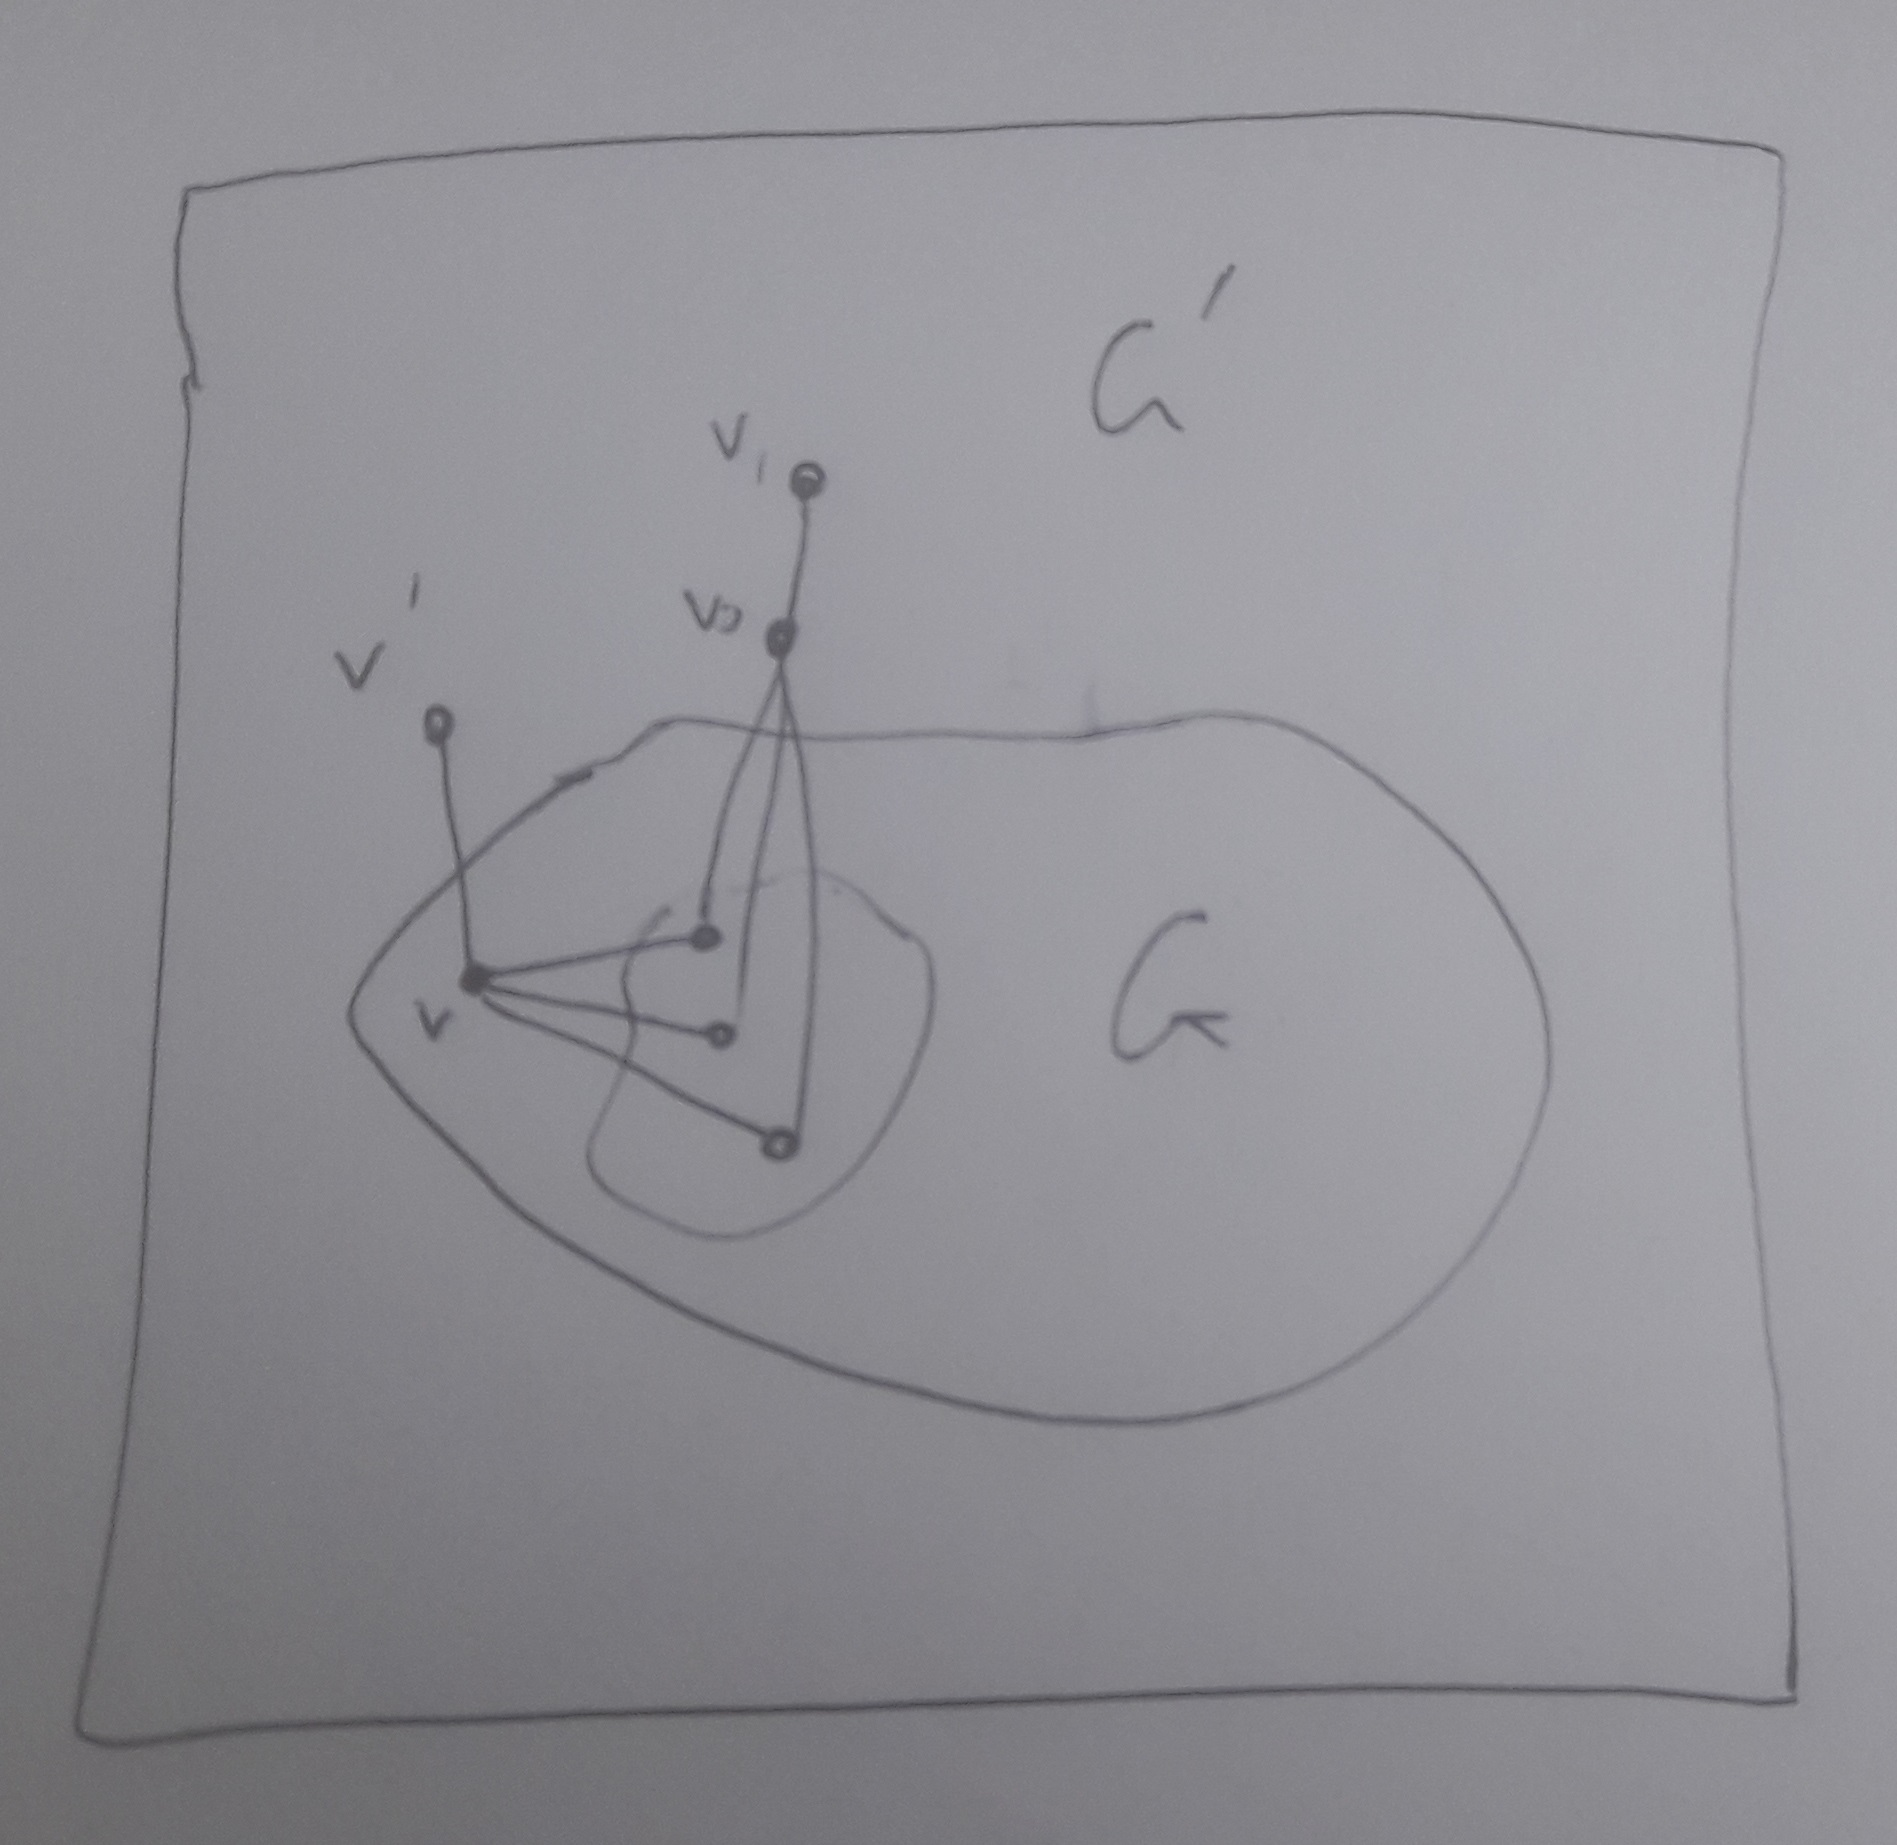
\includegraphics[scale = 0.1]{G.jpg}\]
\end{frame}

\begin{frame}
\frametitle{Q2}
\begin{enumerate}[a)]
\item Show that the construction of $G'$ can be done in polynomial time with respect to $|V|+|E|$. 
\end{enumerate}
\begin{itemize}
\item Assume it takes constant time to choose a vertex $v$, and also that it takes constant time to create vertices. 
\vspace{0.2cm}
\item Then constructing the set of vertices of $G'$ is obviously $O(|V|)$. 
\vspace{0.2cm}
\item We add one edge to $G'$ for every edge of $G$, two edges $\{v,v'\}$ and $\{v_0,v_1\}$, and then an edge $\{v_0,u\}$ for every edge $\{v,u\}$ of $G$. 
\vspace{0.2cm}
\item As usual assuming constant time to create edges, this is $O(|E|) + O(|E|) = O(|E|)$. 
\vspace{0.2cm}
\item So the total time is $O(|V|+|E|)$.
\end{itemize}
\end{frame}

\begin{frame}
\frametitle{Q2}
\begin{enumerate}[b)]
\item Prove that $G$ has a Hamiltonian circuit implies $G'$ has a Hamiltonian path.
\end{enumerate}
\begin{itemize}
\item Let $u_0,\ldots,u_n$ be a Hamiltonian circuit of $G$, and suppose without loss of generality that $u_0 = v$. 
\vspace{0.2cm}
\item Consider the sequence $v',v=u_0,\ldots,u_n,v_0,v_1$ of $G'$. 
\vspace{0.2cm}
\item There are obviously no repeated vertices in this sequence. 
\vspace{0.2cm}
\item There are edges $\{v',v\}$ and $\{v_0,v_1\}$ by construction of $G'$.
\vspace{0.2cm}
\item As there is an edge $\{u_n,u_0\}$ in $G$, there is also an edge $\{u_n, v_0\}$. 
\vspace{0.2cm}
\item It follows that $v',v,u_0,\ldots,u_n,v_0,v_1$ is a Hamiltonian path.
\vspace{0.2cm}
\item So $G$ has a H. circuit implies $G'$ has a H. path.
\end{itemize} 
\end{frame}

\begin{frame}
\frametitle{Q2}
\begin{enumerate}[c)]
\item Prove that $G'$ has a Hamiltonian path implies $G$ has a Hamiltonian circuit.
\end{enumerate}
\begin{itemize}
\item Conversely, suppose $u_0,u_1,\ldots,u_{m-1},u_m$ is a Hamiltonian path in $G'$. 
\item $v'$ and $v_1$ are the only possible endpoints of such a path.
\item So we can suppose without loss of generality that $u_0 = v'$, $u_1 = v$, $u_{m-1} = v_0$ and $u_m = v_1$. 
\item It follows that $u_1,\ldots,u_{m-2}$ is a Hamiltonian path in $G$. 
\item Moreover, as there is an edge $\{u_{m-2},u_{m-1}\}$ in $G'$ (i.e. from $u_{m-2}$ to $v_0$), there must be an edge $\{u_{m-2},u_1\}$ in $G$ (i.e. from $u_{m-2}$ to $v=u_1$). 
\item Thus $u_1,\ldots,u_{m-2}$ is a Hamiltonian circuit as required. 
\item So $G'$ has H. path implies $G$ has H. circuit.
\vspace{0.5cm}
\item That $HCP\leq_p HPP$ follows immediately.
\end{itemize} 
\end{frame}

\end{document}